\documentclass{article}
\setlength{\parskip}{0pt} % esp. entre parrafos
\setlength{\parindent}{3pt} % esp. al inicio de un parrafo
\usepackage{amsmath} % mates
\usepackage{listings}
\usepackage[sort&compress,numbers]{natbib} % referencias
\usepackage{url} % que las URLs se vean lindos
\usepackage[top=15mm,left=20mm,right=20mm,bottom=25mm]{geometry} % \textbf{\textbf{}}margenes
\usepackage{hyperref} % ligas de URLs
\usepackage{graphicx} % poner figuras
\usepackage{subfigure}
\usepackage[spanish]{babel} % otros idiomas
\hypersetup{
    colorlinks=true,
    linkcolor=blue,
    filecolor=blue,      
    urlcolor=blue,
    citecolor=black,
}

\title{TAREA \# 9 \\ Interacciones entre partículas} %titulo
\author{Natalia Berenice P\'{e}rez L\'{o}pez} % author
\date{\today}

\begin{document} % inicia contenido

\maketitle % cabecera

\section{Objetivo}
El objetivo de esta práctica es agregar a cada partícula una masa y hacer que la masa cause fuerzas gravitacionales (atracciones) además de las fuerzas causadas por las cargas. Estudiar la distribución de velocidades de las partículas y verificar gráficamente que esté presente una relación entre los tres factores: la velocidad, la magnitud de la carga, y la masa de las partículas. Tomar en cuenta que la velocidad también es afectada por las posiciones.

\section{Desarrollo} % seccion y etiqueta
Para generar el código de esta práctica se realizaron algunas ideas y pruebas iniciales, las cuales se encuentran en \href{https://github.com/nataliaperez0/Simulation/tree/main/Tarea9}{mi repositorio}  en GitHub. Se inició tomando como base el código revisado en clase para la interacción entre partículas debido a las fuerzas de atracción y repulsión \citep{1}. Las modificaciones que se le realizaron al código fueron: agregar una masa $m$ distribuida normalmente al azar entre $1$ y $3$ a cada una de las $50$ partículas, esta masa se agregó en otra columna del \texttt{data.frame} $p$, también se añadió la columna $vel$ con valores iniciales de $0$ para en su momento almacenar las velocidades de las partículas.
\bigskip

A continuación se muestran las modificaciones del código mencionadas anteriormente:

\definecolor{verde}{rgb}{0,0.56,0.22}
\definecolor{codegray}{rgb}{0.5,0.5,0.5}
\definecolor{codegreen}{rgb}{0,0.56,0.22}
\definecolor{backcolour}{rgb}{0.95,0.95,0.92}
\definecolor{azul}{rgb}{0,0,1}

\lstdefinestyle{mystyle}{
    backgroundcolor=\color{backcolour},   
    commentstyle=\color{verde},
    keywordstyle=\color{azul},
    numberstyle=\tiny\color{codegray},
    stringstyle=\color{codegreen},
    basicstyle=\ttfamily\footnotesize,
    breakatwhitespace=false,         
    breaklines=true,                 
    captionpos=b,                    
    keepspaces=true,                 
    numbers=left,                    
    numbersep=5pt,                  
    showspaces=false,                
    showstringspaces=false,
    showtabs=false,                  
    tabsize=2
}

\lstset{style=mystyle}
\begin{lstlisting}[language=R, caption= Código para agregar la masa $m$ con valores distribuidos normalmente al azar entre $1$ y $3$ .]
n <- 50
p <- data.frame(x = rnorm(n), y=rnorm(n), c=rnorm(n), m=rnorm(n), vel = numeric(n))
xmax <- max(p$x)
xmin <- min(p$x)
p$x <- (p$x - xmin) / (xmax - xmin) # ahora son de 0 a 1
ymax <- max(p$y)
ymin <- min(p$y)
p$y <- (p$y - ymin) / (ymax - ymin) # las y tambien son de 0 a 1
cmax <- max(p$c)
cmin <- min(p$c)
p$c <- 2 * (p$c - cmin) / (cmax - cmin) - 1 # cargas son entre -1 y 1
p$g <- round(5 * p$c) # coloreamos segun la carga a 11 niveles de -5 a 5
mmax = max(p$m) 
mmin = min(p$m)
p$m = (2 * (p$m - mmin) / (mmax - mmin) + 1) #masa entre 1 y 3
paso <- floor(256 / 10)
niveles <- seq(0, 255, paso)
colores <- rgb(niveles, rep(0, 11), rev(niveles), max=255)
eps <- 0.001
\end{lstlisting}

Posteriormente en la función \texttt{fuerza} del código se realizaron las siguientes modificaciones con apoyo del repositorio de Claudia Hernández \citep{2} para obtener la fuerza gravitatoria $F_G$ generada por la masa $m$ de las partículas: dado que la $F_G$ en la vida real esta dada por la ecuación \ref{eq:e1} (ley de gravitación universal), donde: $G= 6.674\times10^{-11}$ (constante de gravitación universal) se utilizó está misma ecuación \ref{eq:e1} para calcular la fuerza gravitatoria de las partículas en $x$ y en $y$, para así después sumarla a las fuerzas de atracción y repulsión. Se utilizó como constante de gravitación universal el valor de $G = 0.6674$ debido a que el valor real de esta constante es muy pequeño para apreciar efectos significativos.
 
\begin{equation}
\label{eq:e1}
F_G= G\frac{m_1 m_2}{r^{2}} 
\end{equation}

\newpage

\lstset{style=mystyle}
\begin{lstlisting}[language=R, caption= Código para generar fuerzas gravitacionales debido a la masa de las partículas.]
G <- 0.6674 #valor supuesto para la constante gravitacional(6.674*10^(-11))

fuerza <- function(i) { 
  xi <- p[i,]$x
  yi <- p[i,]$y
  ci <- p[i,]$c
  mi = p [i,]$m
  fx1 = 0
  fy1 = 0
  fx2 = 0
  fy2 = 0
  for (j in 1:n) {
    cj <- p[j,]$c
    mj = p[j,]$m
    dir <- (-1)^(1 + 1 * (ci * cj < 0)) #es atraccion o repulsion
    dx <- xi - p[j,]$x
    dy <- yi - p[j,]$y
    factor <- dir * abs(ci - cj) / (sqrt(dx^2 + dy^2) + eps) 
    fg <- G * ((mi * mj) / ((sqrt(dx^2 + dy^2) + eps)^2)) #fuerza gravitatoria
    fx1 = fx1 - dx * factor
    fy1 = fy1 - dy * factor
    fx2 = fx2 - dx * fg
    fy2 = fy2 - dy * fg
    #sumatoria de fuerzas
    fx = fx1 + fx2
    fy = fy1 + fy2
  }
  return(c(fx, fy))
}
\end{lstlisting}

En el experimento se realizaron $100$ pasos y se graficaron para visualizar el movimiento de las partículas, también se cálculo la velocidad tomando en cuenta la \texttt{fuerza resultante} $F_R$ dada por la ecuación \ref{eq:e2} y se almacenaron éstos datos en el \texttt{data.frame} $p$.

\begin{equation}
\label{eq:e2}
F_R= \sqrt{{F_x^{2} +F_y^{2}}} 
\end{equation}

\lstset{style=mystyle}
\begin{lstlisting}[language=R, caption= Código para obtener la velocidad de cada partícula.]
suppressMessages(library(doParallel))
registerDoParallel(makeCluster(detectCores() - 1))
tmax <- 100
digitos <- floor(log(tmax, 10)) + 1
tl <- "0"
while (nchar(tl) < digitos) {
  tl <- paste("0", tl, sep="")
}
png(paste("p9_t", tl, ".png", sep=""))
plot(p$x, p$y, col=colores[p$g+6], pch=16, cex=p$m, xlim=c(-0.1, 1.1), ylim=c(-0.1, 1.1),
     main="Estado inicial", xlab="X", ylab="Y")
graphics.off()
for (iter in 1:tmax) {
  f <- foreach(i = 1:n, .combine=c) %dopar% fuerza(i)
  delta <- 0.02 / max(abs(f)) # que nadie desplace un paso muy largo
  p$x <- foreach(i = 1:n, .combine=c) %dopar% max(min(p[i,]$x + delta * f[c(TRUE, FALSE)][i], 1), 0)
  p$y <- foreach(i = 1:n, .combine=c) %dopar% max(min(p[i,]$y + delta * f[c(FALSE, TRUE)][i], 1), 0)
  v = foreach(i = 1:n, .combine=c)%dopar% sqrt((delta * f[c(TRUE, FALSE)][i])^2 + (delta * f[c(FALSE, TRUE)][i])^2)
  p$vel = p$vel+v
\end{lstlisting}

En la figura \ref{f1} se muestran algunas gráficas del movimiento de las partículas, se puede observar que conforme pasan las iteraciones las partículas experimentan fuerzas de atracción y la mayoría se reúne en un mismo punto debido a éstas fuerzas. 
\bigskip

Se realizó un gif \citep{3} con los $100$ pasos del movimiento de las partículas, el cual se encuentra en \href{https://github.com/nataliaperez0/Simulation/tree/main/Tarea8}{mi repositorio} en GitHub.

\newpage

\begin{figure}[h!]
\centering
\subfigure[Paso = 0]{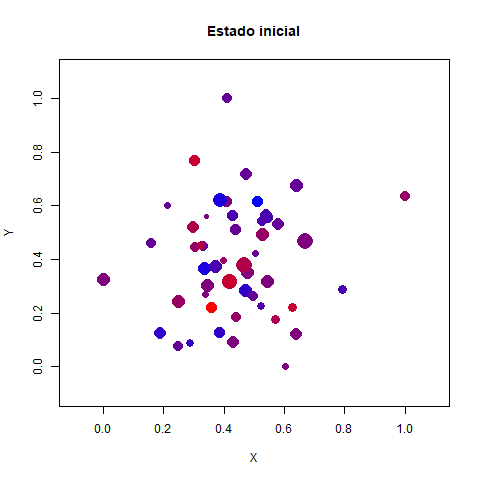
\includegraphics[width=87mm]{Figura1.png}}
\subfigure[Paso = 25]{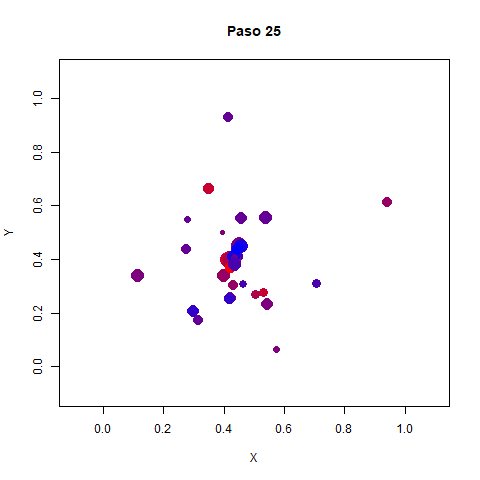
\includegraphics[width=87mm]{Figura2.png}}
\subfigure[Paso = 50]{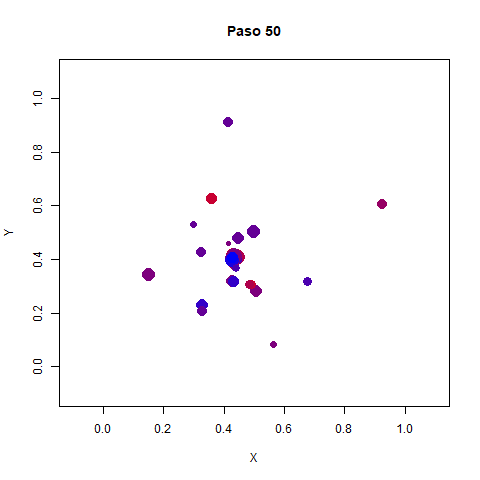
\includegraphics[width=87mm]{Figura3.png}}
\subfigure[Paso = 75]{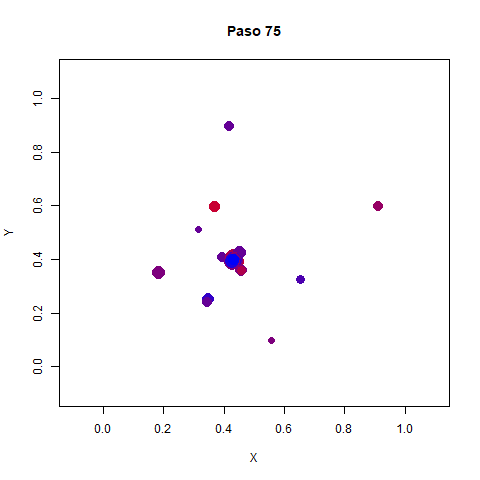
\includegraphics[width=87mm]{Figura4.png}}
\caption{Movimiento de las partículas debido a las fuerzas gravitatorias y a las fuerzas de atracción y repulsión.} 
\label{f1}
\end{figure}

Para visualizar y analizar la relación entre los factores de velocidad, carga y masa de las patículas se realizó el gráfico que se muestra en la figura \ref{f2}. Se puede observar que conforme aumenta la masa $m$ de las partículas también aumenta su velocidad, pero con respecto a la carga no se observa ningún comportamiento específico, podemos notar que partículas con masa y velocidad grande pueden tener una carga positiva, negativa o neutra y lo mismo sucede con partículas con masa y velocidad pequeña.
\bigskip

Para analizar si existe una relación entre la masa y la velocidad de las partículas se realizó una prueba estadística. Para realizar esta prueba se tuvieron algunas dificultades pero con apoyo de mi compañero Eduardo Navarro se logró realizar. Para la prueba estadística se realizaron las siguientes modificaciones en el código objetivo de la tarea: se agregó un ciclo \texttt{for} para variar la masa en valores específicos de $1$ a $3$ en pasos de $0.5$ y para cada masa se realizaron $15$ réplicas del experimento utilizando otro ciclo \texttt{for}, los resultados se almacenaron en un \texttt{data.frame} para posteriormente realizar un diagrama caja-bigote y analizar los resultados. Después de la figura \ref{f2} se muestra el código de las modificaciones mencionadas y en \href{https://github.com/nataliaperez0/Simulation/tree/main/Tarea8}{mi repositorio} se puede encontrar el código completo:

\begin{figure} [h!]% figura
    \centering
    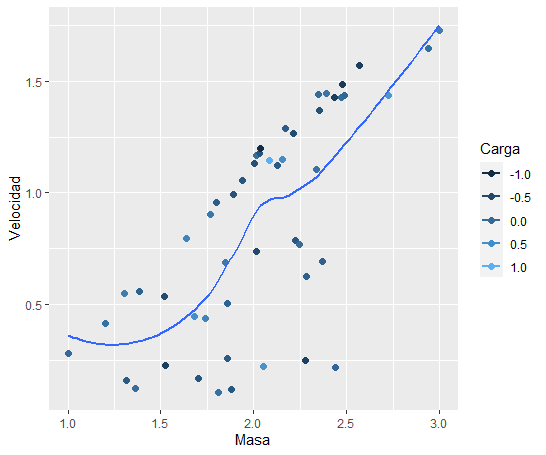
\includegraphics[width=150mm]{Figura5.png} % archivo
    \caption{Relación de la masa, velocidad y carga de las partículas.}
    \label{f2}
\end{figure}

\lstset{style=mystyle}
\begin{lstlisting}[language=R, caption= Código para analizar masas fijas de $1$ a $3$ en pasos de $0.5$ y hacer $15$ réplicas del experimento para cada masa.]
df = data.frame()
masas = seq(1, 3, 0.5)

for (masa in masas){
  for ( replica in 1:15){
    n <- 50
    p <- data.frame(x = rnorm(n), y=rnorm(n), c=rnorm(n), m=rnorm(n), vel = numeric(n))
    xmax <- max(p$x)
    xmin <- min(p$x)
    p$x <- (p$x - xmin) / (xmax - xmin) # ahora son de 0 a 1
    ymax <- max(p$y)
    ymin <- min(p$y)
    p$y <- (p$y - ymin) / (ymax - ymin) # las y tambien son de 0 a 1
    cmax <- max(p$c)
    cmin <- min(p$c)
    p$c <- 2 * (p$c - cmin) / (cmax - cmin) - 1 # cargas son entre -1 y 1
    p$g <- round(5 * p$c) # coloreamos segun la carga a 11 niveles de -5 a 5
    mmax = max(p$m) 
    mmin = min(p$m)
    p$m=masa #masa fija
    paso <- floor(256 / 10)
    niveles <- seq(0, 255, paso)
    colores <- rgb(niveles, rep(0, 11), rev(niveles), max=255)
    eps <- 0.001
    G <- 0.6674 #valor supuesto para la constante gravitacional(6.674*10^(-11))
\end{lstlisting}

En la figura \ref{f3} se muestra el diagrama caja-bigote de los resultados del experimento. Se puede observar que no existen grandes diferencias entre las velocidades obtenidas para cada masa, para analizar mejor los resultados se realizó la prueba estadística.

\begin{figure} [h!]% figura
    \centering
    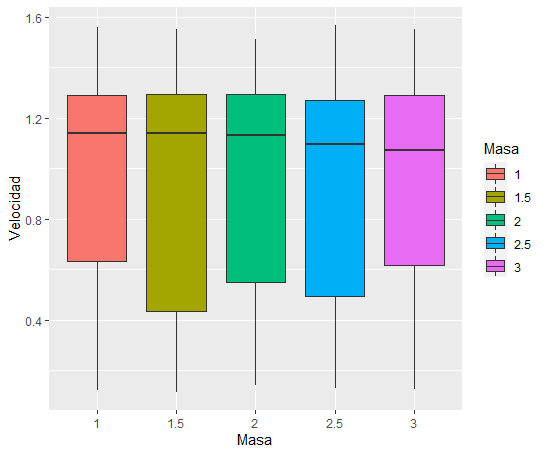
\includegraphics[width=150mm]{Figura6.png} % archivo
    \caption{Velocidad que alcanzan las partículas para cada masa.}
    \label{f3}
\end{figure}

Debido a los resultados obtenidos al revisar la normalidad de los datos, se eligió realizar la prueba estadística \texttt{Kruskal Wallis}. En el cuadro \ref{Cuadro1} se  resumen los resultados de la revisión de los supuestos para poder aplicar la prueba estadística. El supuesto outliers se refiere a la cantidad de valores atípicos que existen en los grupos, la normalidad por grupos se obtuvo con la prueba de \texttt{Shapiro Wilk} y la homogeneidad de varianza se obtuvo con la prueba de \texttt{Levene}.

\begin{table}[h!]
\centering
\caption{Resultados del los supuestos para aplicar la prueba estadística.}
\smallskip

\begin{tabular}{ |p{2.1cm}|p{3.5cm}|}
 \hline
 Outliers & $0$ \\
 \hline
 Normalidad por grupo & $1.00$: $p$ = $3.71\times 10^{-24}$ $1.50$: $p$ = $4.75\times 10^{-26}$ $2.00$: $p$ = $3.02\times 10^{-25}$ $2.50$: $p$ = $1.44\times 10^{-24}$ $3.00$: $p$ = $1.03\times 10^{-23}$\\
 \hline
 Homogeneidad de varianza & $p$ = $0.294$ \\
 \hline
\end{tabular}
\label{Cuadro1}
\end{table}

En los resultados se observa que para la normalidad por grupos todos valores de $p$ son menores a $0.05$, por lo tanto no se tiene normalidad. Al realizar la prueba estadística \texttt{Kruskal Wallis} se obtienen los resultados mostrados en el cuadro \ref{Cuadro2}.

\begin{table}[h!]
\centering
\caption{Resultados al aplicar la prueba estadística \texttt{Kruskal Wallis}.}
\smallskip

\begin{tabular}{ |p{2.1cm}|p{2.1cm}|}
 \hline
 Chi cuadrada & Valor de $p$ \\
 \hline
 $7.1106$ & 0.1302 \\
 \hline
\end{tabular}
\label{Cuadro2}
\end{table}

Hipótesis nula : Las medias son iguales en todos los grupos.
\smallskip

Debido a que $p > 0.05$ se acepta la hipótesis nula, es decir que no existen diferencias significativas entre las medias de los grupos. Se entiende entonces que la variación de la masa $m$ de las partículas no tiene un efecto significativo en la velocidad de las mismas.
\bigskip

También podemos realizar la prueba de suma de rangos de \texttt{Wilcoxon} por pares para observar los resultados de $p$ y determinar si existen diferencias al comparar entre ellas las masas (Ver cuadro \ref{Cuadro3}).

\begin{table}[ht]
\centering
\caption{Resultados al aplicar la prueba \texttt{Wilcoxon}.}
\smallskip

\begin{tabular}{|p{1.7cm}|p{1.7cm}|p{1.7cm}|p{1.7cm}|p{1.7cm}|}
 \hline
Valor de $p$ & $1.00$ & $1.50$ & $2.00$ & $2.50$ \\
 \hline
 $1.50$ & $1$ & - & - & -  \\
 \hline
 $2.00$ & $1$ & $1$ & - & -  \\
 \hline
 $2.50$ & $0.15$ & $1$ & $1$ & -  \\
 \hline
 $3.00$ & $0.44$ & $1$ & $1$ & $1$  \\
 \hline
\end{tabular}
\label{Cuadro3}
\end{table}

En los resultados de la prueba podemos observar que todos los valores de $p$ son mayores a $0.05$, lo cual indica que no existen diferencias significativas entre sus medias.
\bigskip

A continuación se muestra el código utilizado para realizar la prueba estadística \texttt{Kruskal Wallis}:

\lstset{style=mystyle}
\begin{lstlisting}[language=R, caption= Código para las pruebas estadísticas \texttt{Kruskal Wallis} y \texttt{Wilcoxon}.]
library(tidyverse)
library(ggpubr)
library(car)
library(rstatix)
library(rapportools)
library(readr)
library(gridExtra)

#PRUEBA ESTADISTICA...
#Estadisticas descriptivas
df %>%
  group_by(Masa) %>%
  get_summary_stats(Velocidad, type = "mean_sd")
#SUPUESTOS PARA ANOVA
#1:Outliers
df %>%
  group_by(Masa) %>%
  identify_outliers(Velocidad)
#2:Normalidad por Shapiro
df %>%
  group_by(Masa) %>%
  shapiro_test(Velocidad)
#3:Homogeneidad de varianza con prueba Levene
df %>%
  levene_test(Velocidad~Masa)
#PRUEBA ESTADISTICA KRUSKAL WALLIS
kruskal.test(Velocidad ~ Masa, data = df)
#PRUEBA WILCOXON
pairwise.wilcox.test(df$Velocidad, df$Masa)
\end{lstlisting}

\newpage
\section{Conclusi\'{o}n}
Con base en los resultados de la relación entre la masa, velocidad y carga de las partículas mostrados en la figura  \ref{f2} puedo concluír que cuando se asignan masas distribuidas normalmente al azar la velocidad resultante debida a las fuerzas de las cargas y a las fuerzas gravitatorias aumenta cuando se aumenta la masa también, esto como consecuencia de que tienen una mayor fuerza para moverse, además en la figura \ref{f2} se puede observar que no existe una relación directa en la carga que presentan las partículas. Con respecto a la prueba estadística aplicada se puede observar en el diagrama caja-bigote que cuando se asigna una masa fija para el experimento no se presentan cambios significativos en las velocidades de cada masa fija, para observar la relación entre la masa y la velocidad es necesario tener una experimento con masas distribuidas normalmente al azar.
\smallskip

En general ésta práctica se me dificultó un poco en la parte estadística pero con el apoyo de mis compañeros finalmente pude realizarla.
\newpage

\bibliography{referencias}
\bibliographystyle{plainnat}

\end{document}